\problem{}
(a) The Laplacian kernel is that:
$$
\nabla^2 f = \begin{bmatrix}
    0 & 1 & 0 \\
    1 & -4 & 1 \\
    0 & 1 & 0
\end{bmatrix}
=
\begin{bmatrix}
    0 & 1 & 0 \\
    0 & -2 & 0 \\
    0 & 1 & 0
\end{bmatrix}
+
\begin{bmatrix}
    0 & 0 & 0 \\
    1 & -2 & 1 \\
    0 & 0 & 0
\end{bmatrix}
$$
We can seperate the Laplcian kernel along the $x$-direction and $y$-direction, and we can simplify them into 1-D:

$$\begin{bmatrix}1\\-2\\1\end{bmatrix} \text{\ \ and \ \ } \begin{bmatrix}1 & -2 & 1\end{bmatrix}$$

The processed image corresponding to the kernel above all shown in Figure \ref{fig:p2a}.\\

\begin{figure}[htbp]
    \centering
	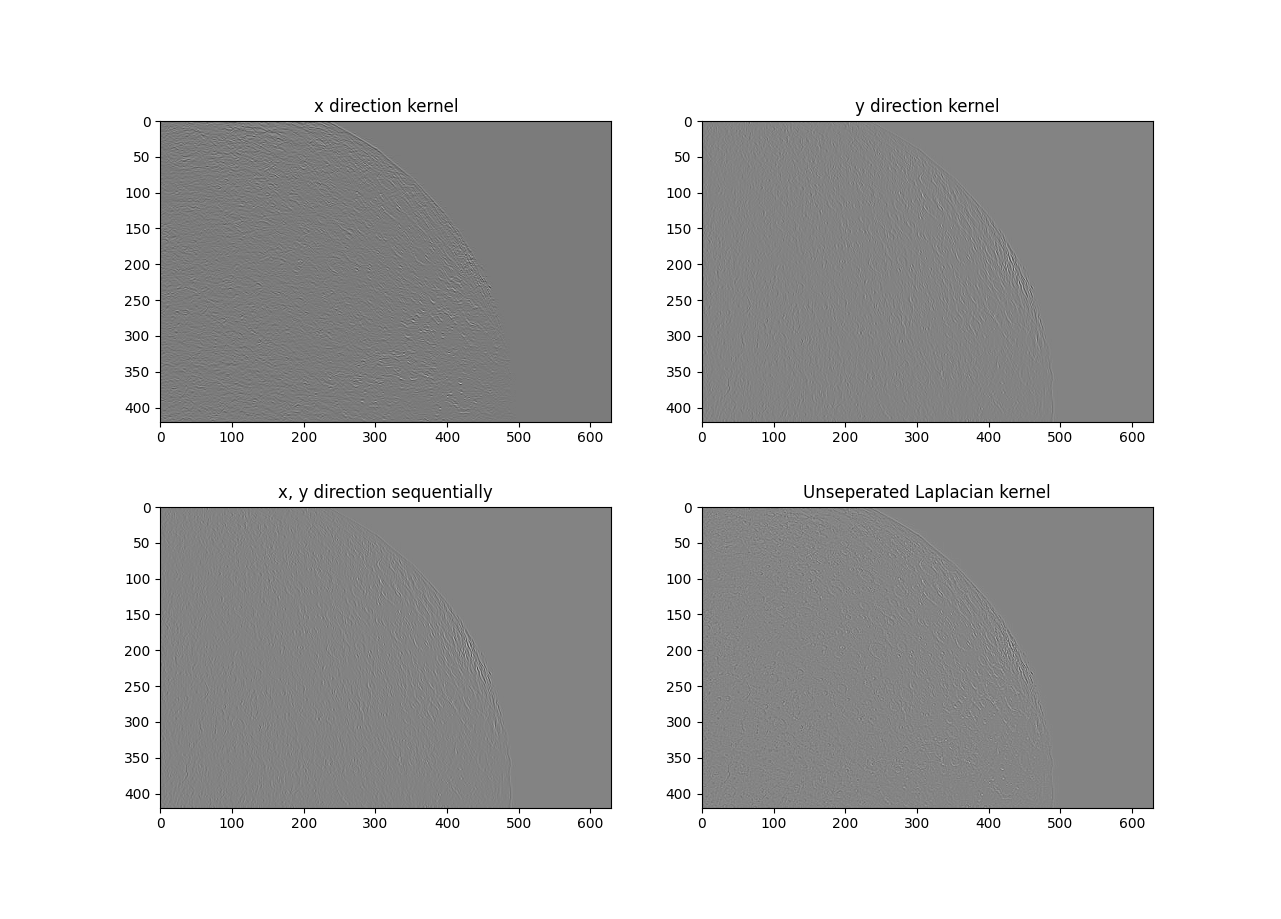
\includegraphics[width=1\textwidth]{../images/p2/p2a.png}
    \caption{Separated Laplacian kernels processed image}
\label{fig:p2a}
\end{figure}


(b) The Sharpened image with Laplacian kernel is shown in Figure \ref{fig:p2b}.\\
\begin{figure}[htbp]
    \centering
    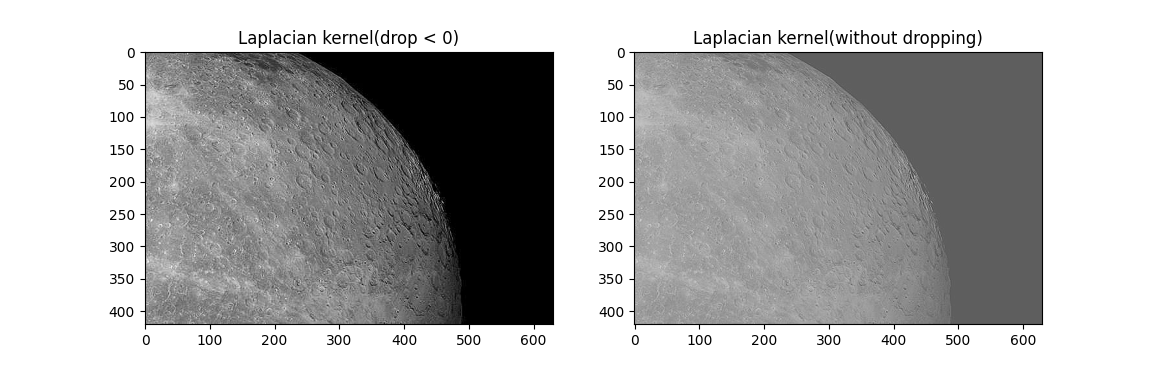
\includegraphics[width=\textwidth]{../images/p2/p2b.png}
    \caption{Unseparated Laplacian kernel processed image}
\label{fig:p2b}
\end{figure}

The image sharpening with Laplacian could be seen as sharpened with the kernel
$$
\begin{bmatrix}
    0 & -1 & 0 \\
    -1 & 5 & -1 \\
    0 & -1 & 0
\end{bmatrix}
$$

In order to make the right side of the image to be black instead of being gray, the $<0$ and $>255$ part are abandoned, i.e. turning the $<0$ part into $0$, and turning the $>255$ part into $255$,
which is shown in the left image.\\
And the right image is doing no additional operations, slighting mapping $[\text{min},\text{max}]\to[0,255]$.\\

(c) The Sharpened image with unsharpen mask is shown in Figure \ref{fig:p2c}.\\
The first two rows (marked filter1 in the title) are smoothed with the kernel 
$$\text{kernel\ 1}=\dfrac{1}{9}\begin{bmatrix}1 & 1 & 1\\1 & 1 & 1\\1 & 1 & 1\end{bmatrix}$$

And the last two rows (marked filter2 in the title) are smoothed with the kernel
$$\text{kernel\ 2}=\dfrac{1}{16}\begin{bmatrix}1 & 2 & 1\\2 & 4 & 2\\1 & 2 & 1\end{bmatrix}$$

Suppose the origin image is $f(x,y)$.\\
The first column are the smoothed images processed by kernel1 and kernel2, mark as $\overline{f(x,y)}$.\\
The second column are the unsharped masks processed by kernel1 and kernel2. i.e. the difference between the
origin image and the smoothed image. i.e. $g_{mask}(x,y)=f(x,y)-\overline{f(x,y)}$.\\
The third and the forth column are the sharpened images with different $k$. i.e. $g(x,y)=f(x,y)+k\cdot g_{mask}(x,y)$\\
The third column is the sharpened image with $k=1$, and the forth column is the sharpened image with $k=4.5$.\\
And the fifth column is the origin image.\\

For the difference bewteen the $1,2$ rows and $3,4$ rows is that: the $1,3$ rows are doing normalization with $[\text{min},\text{max}]\to[0,255]$,
and the $2,4$ rows are setting $<0$ and $>255$ part are abandoned, i.e. turning the $<0$ part into $0$, and turning the $>255$ part into $255$.\\
We could see that as $k$ grows, more high frequency of the image increases, make the image sharper.\\

\begin{figure}[htbp]
    \centering
	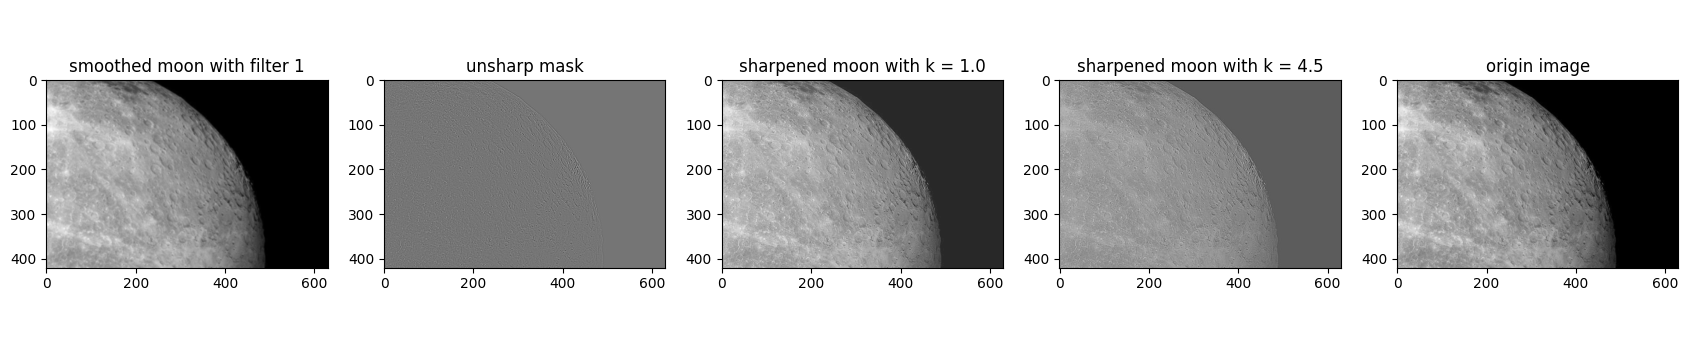
\includegraphics[width=\textwidth]{../images/p2/p2c_1_no_drop.png}
	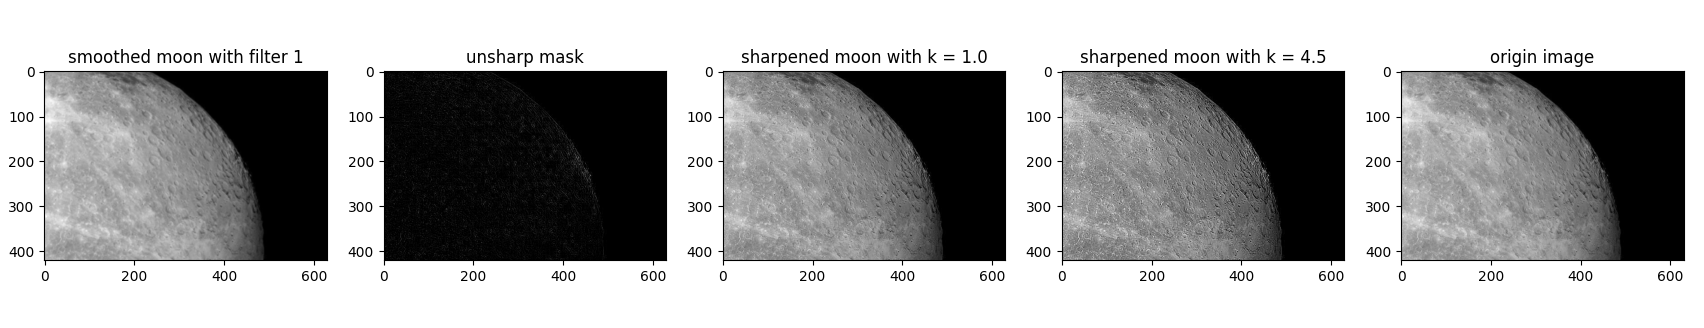
\includegraphics[width=\textwidth]{../images/p2/p2c_1_drop.png}
    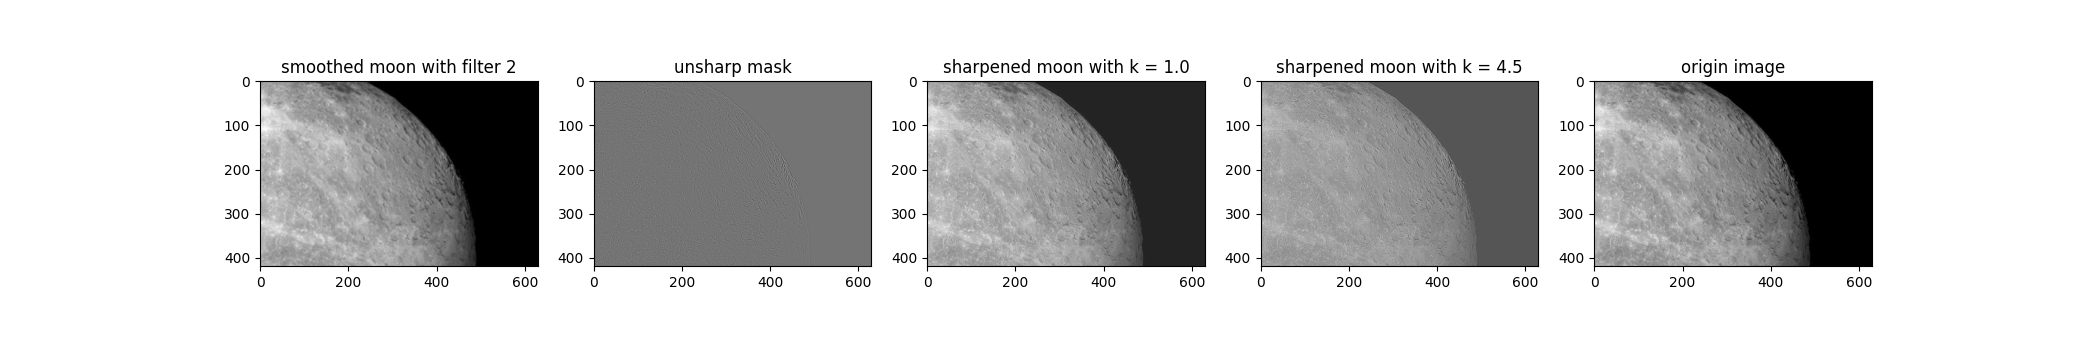
\includegraphics[width=\textwidth]{../images/p2/p2c_2_no_drop.png}
	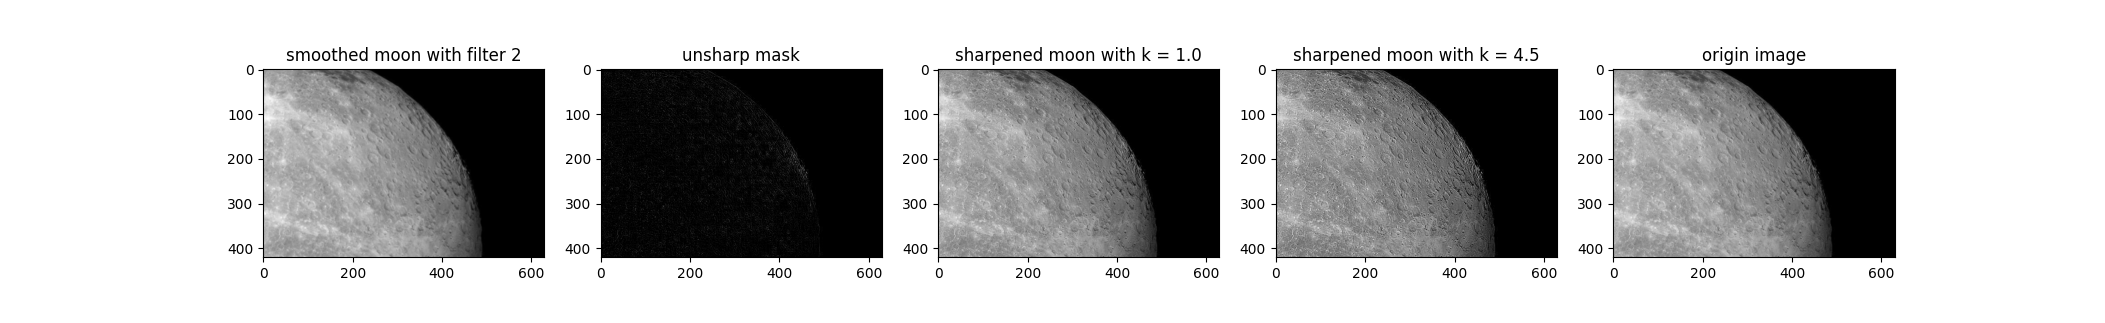
\includegraphics[width=\textwidth]{../images/p2/p2c_2_drop.png}
    \caption{unsharpen mask processed image}
\label{fig:p2c}
\end{figure}

\newpage